%----------------------------------------------------------------------------------------------------------------------------------------------------------%
\chapter{Physical experimentation}
\epigraph{A scientist in his laboratory is not a mere technician: he is also a child confronting natural phenomena that impress him as though they were fairy tales.}{\textit{Marie Curie}}
%----------------------------------------------------------------------------------------------------------------------------------------------------------%
\section{Description}
\paragraph{}This experiment looks at finding out the prevalence of \emph{Staphylococcus aureus} in a sample of students from the school. The process used involves extracting a sample from underneath a subject's nalis by swabbing, cultivating that sample and then observing the results of said culture to determine the presence or not of \emph{Staphylococcus aureus} as part of the subject's resident bacterial flora. Each iteration of the process took less than two minutes to complete. However, all the safety measures and actions taken need more time to be taken care of properly.
%----------------------------------------------------------------------------------------------------------------------------------------------------------%
\section{Protocol followed}
\paragraph{}The protocol followed was designed based on a similar protocol used in the many university laboratories\cite{olearyPracticalHandbookMicrobiology1989}, modified to fit the needs of this research paper, and peer-reviewed by Olga Sánchez, and uploaded to the Protocols.io platform, to make it easier to follow the days of that the experiment took place in. This protocol underwent 9 different revisions\cite{rocacugatStaphilococcusAureusSampling2022a}. It can also be read below:
\begin{enumerate}[label=\arabic*)]
\item Prepare yourself for the experimentation: wash your hands, put on gloves, put on the lab coat, mask and goggles. Wash your hands again (gloves still on). Set up the work area; the Bunsen burner should be turned on in such a way that it can cover an acceptable surface to work. Turn it on and wash your hands again.
\item Divide each Petri dish between 2 parts. A guide should be used for this part. Get your subject to wash their hands. Observe their hands. If they are extremely short, it may be worth it to take the sample nasally.
\item Note down their information, crack open a sterile swab, dip it in Ringer solution and swab away at under their nails or nose. Then, populate the dish with this sample.
\item Incubate for 32-48h and observe the results.
\item Observe the bacteria under a microscope after GRAM tinction.
\end{enumerate}
%----------------------------------------------------------------------------------------------------------------------------------------------------------%
\section{Bill of materials}
\paragraph{}The materials used, as well as the quantities used can be found in the following table. On the left, laboratory equipment and, on the right, reagents, tinction agents, and consumables used:
\begin{center}\begin{figure}[H]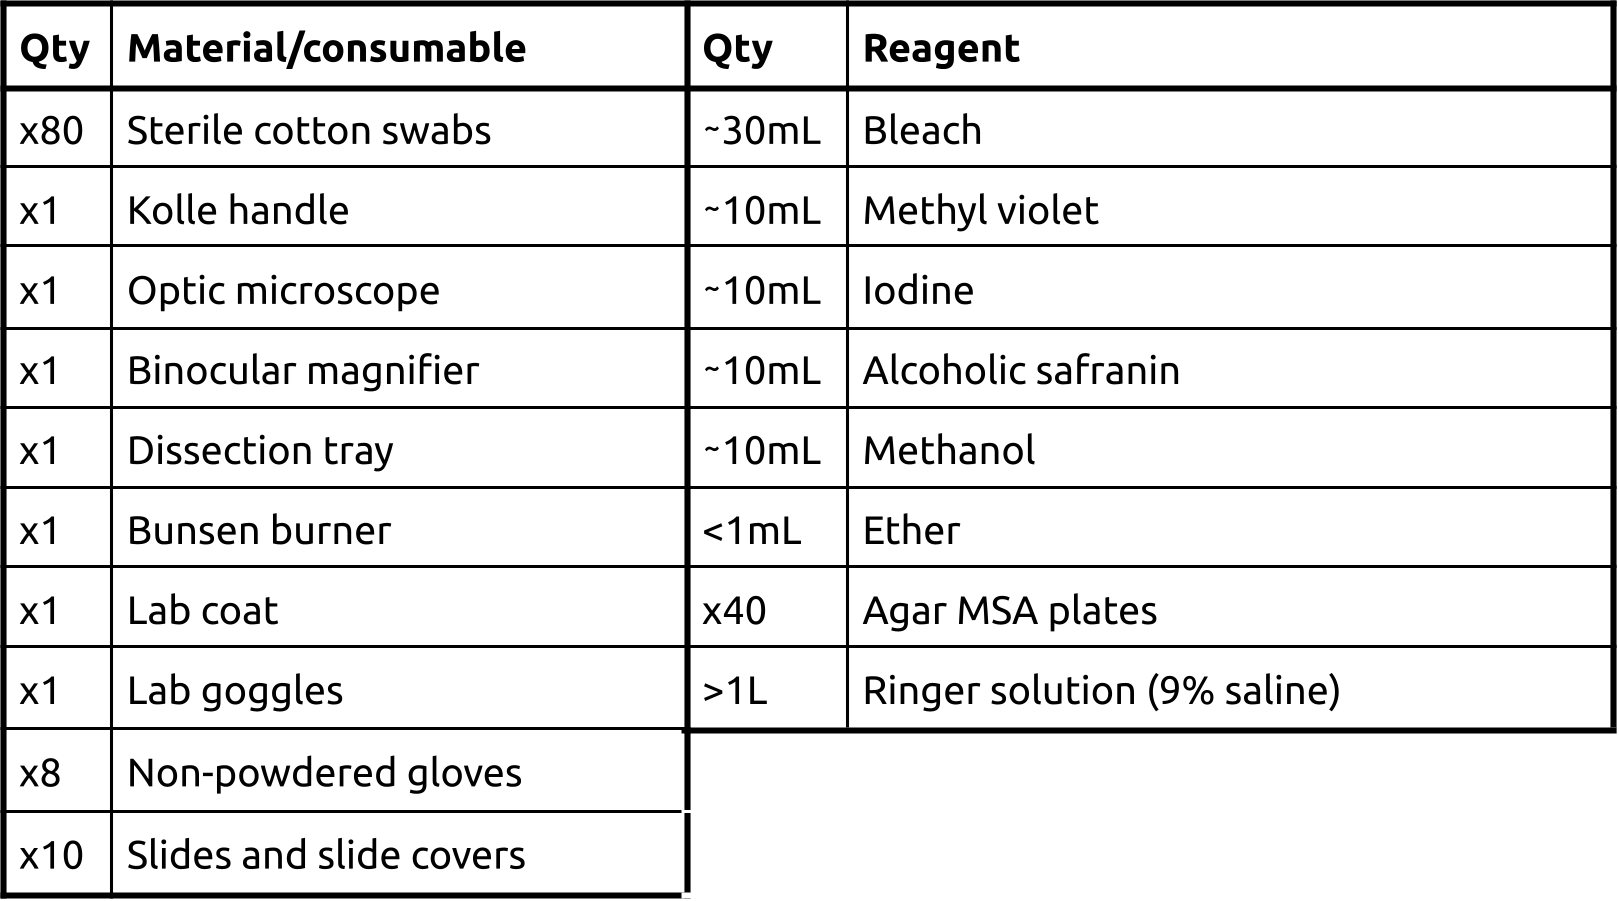
\includegraphics[width=0.90\textwidth]{BOM-1.png}\end{figure}\end{center}
%----------------------------------------------------------------------------------------------------------------------------------------------------------%
\section{Biosecurity and risk mitigation}
\paragraph{}Staph is considered a Biosecurity Level (BSL) 2 pathogenic bacteria\cite{cheungPathogenicityVirulenceStaphylococcus2021}. This means that the it is associated with a human disease that can pose a moderate human health hazard. In a laboratory where BSL-2 pathogens are handled, regular lab rules should be followed (mechanical pipetting only, hand washing, prohibition of the consumption of food and drinks in the lab, proper PPE use...), as well as avoiding splashes or aerosols, adhering biohazard warning signs present on all material used, as well as proper surface and material disinfection via the use of autoclave or proper alternative decontamination method\cite{worldhealthorganizationLaboratoryBiosafetyManual2020}.\newline
The risks associated with this bacteria were assessed following the protocol designated by the World Health Organisation, and proper security measures were followed at all times when handling biohazardous material. No incidents occurred during the research part of this project, and the protocol defined previous to the start was followed extremely closely. While the laboratory used may not be the most ideal type of laboratory for this type of research, it was certainly adequate enough to perform a research project like this one, especiallly after the temporary signage that was temporarily installed.
%----------------------------------------------------------------------------------------------------------------------------------------------------------%
\section{Results and analysis}
The results obtained can be found as Annex II in the form of a raw data table with personal identificative data removed following GDPR regulations. The data was then recounted and graphed into the following pie chart:
\begin{center}\begin{figure}[h!]  \centering\begin{subfigure}[b]{0.4\linewidth}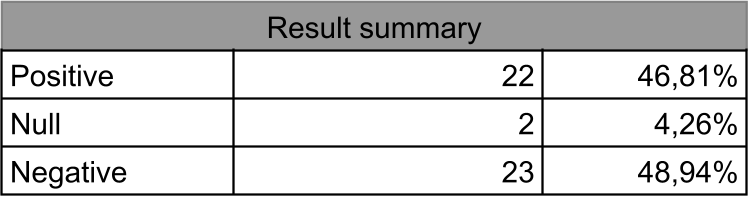
\includegraphics[width=\linewidth]{Data.png}\caption{Counts of the result cases. Own data.}\end{subfigure}\begin{subfigure}[b]{0.4\linewidth}\includegraphics[width=\linewidth]{Pie.png}\caption{Pie graph of the result cases. Own data.}\end{subfigure}\end{figure}\end{center}
As we can see, almost 50\% of the samples taken tested positive for \emph{Staphylococcus aureus}, compared to the expected 30\%\cite{StaphylococcusAureusHealthcare2020}. We can, however, see in the UK's Public Health bactaeremia data that Staph infections have been on the rise lately, so it may not be a case of wrong data\cite{englandMSSABacteraemiaAnnual2021}. On top of that, both of my advisers, Olga and Margarita, have also found themselves getting more prevalence than usual of this bacteria, and are finding cases that were once negative but turned positive in the last few years. \footnote{insert table}
\paragraph{}There may be several reasons for the infection rate and thus natural prevalence to be increasing. One of them could be that since antibiotic abuse is growing with each passing year, the usual resident microbiota is getting killed, leaving more resources for Staph to thrive in that environment. To confirm this theory we will look at the infection rates of a country that is facing extreme antibiotic abuse (the United States of America) and compare it to another that is controlling their antibiotics a bit better (the United Kingdom). They have seen a 210\% increase in \emph{Staphylococcus aureus} cases since 2006. However, superfluous antibiotic prescriptions have increased by barely 1\%\cite{baggsEstimatingNationalTrends2016}. In the United Kingdom, they have seen a 160\% increase in \emph{Staphylococcus aureus} infections\cite{englandMSSABacteraemiaAnnual2021}, and their superfluous antibiotic prescriptions have gone down by 20\%. While this seems like very little data to extract conclusions from, it is clear that there may be a correlation between these two factors.
\paragraph{}The other could be climate change. An increase of ambient temperatures could mean a better breeding ground for this specific species and thus leading to a higher-than-usual prevalence. \emph{Staphylococcus aureus}' optimal breeding temperature is between 35\si{\celsius} and 37\si{\celsius}. The global average temperature has increased by 1,1\si{\celsius}\cite{gmsGMSAnnualGlobal2016} in the last 120 years. And \emph{Staphylococcus aureus} has a specific temperature growth curve, just like any other bacteria:\newline\begin{center}\begin{figure}[H]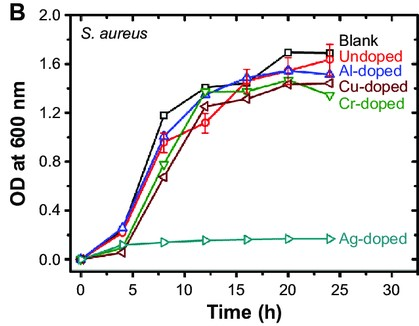
\includegraphics[width=0.76\textwidth]{tempcurve.png}\caption{\emph{Staphylococcus aureus} growth curve by temperature\cite{FigEffectTemperature2022}}\end{figure}\end{center} So, this correlation may not be completely incorrect, and in fact some scientists warn aobut an increased number of infectious diseases resurging due to climate change. One only data point is not enough significant data, so further study is needed on this front.
\paragraph{}[bacteria observation] [this failed so i'm repeating it on thursday at UdG]
